\fontfamily{\sfdefault}\selectfont
% XCircuit output "leeson_pn.tex" for LaTeX input from leeson_pn.ps
\def\putbox#1#2#3#4{\makebox[0.00000in][l]{\makebox[#1][l]{}\raisebox{\baselineskip}[0.00000in][0.00000in]{\raisebox{#2}[0.00000in][0.00000in]{\scalebox{#3}{#4}}}}}
\def\rightbox#1{\makebox[0.00000in][r]{#1}}
\def\centbox#1{\makebox[0.00000in]{#1}}
\def\topbox#1{\raisebox{-0.60\baselineskip}[0.00000in][0.00000in]{#1}}
\def\midbox#1{\raisebox{-0.20\baselineskip}[0.00000in][0.00000in]{#1}}
   \scalebox{1}{
   \normalsize
   \parbox{2.68750in}{
   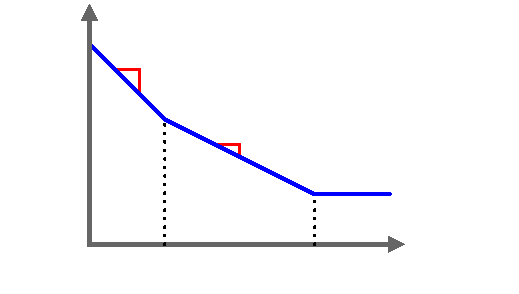
\includegraphics[scale=0.80000]{./figs/leeson_pn.pdf}\\
   % translate x=-248 y=245 scale 0.38
   \putbox{1.88000in}{0.06400in}{0.90}{$\log(\Delta f)$}%
   \putbox{0.80800in}{1.23200in}{0.72}{-30 dB/dec}%
   \putbox{0.80800in}{1.09600in}{0.72}{$\propto f^{-3}$}%
   \putbox{1.34400in}{0.73600in}{0.72}{$\propto f^{-2}$}%
   \putbox{1.34400in}{0.86400in}{0.72}{-20 dB/dec}%
   \putbox{0.80800in}{0.13600in}{0.72}{\rotatebox{-360}{$f_1$}}%
   \putbox{1.60800in}{0.13600in}{0.72}{\rotatebox{-360}{$f_2$}}%
   \putbox{0.04800in}{1.40000in}{0.90}{$\mathcal{L}(\Delta f)$}%
   } % close 'parbox'
   } % close 'scalebox'
   \vspace{-\baselineskip} % this is not necessary, but looks better
\fontfamily{\rmdefault}\selectfont
